\chapter{La gestion de projets}
\section{L'équipe projet}
Clarisys Informatique est une entreprise mêlant des personnes issues du domaine de 
l’informatique et de la biologie médicale. Elle est divisée en deux équipes principales 
qui collaborent sur la production de deux logiciels commercialisés par l’entreprise, 
auxquelles s’ajoutent la direction et l’administration, les chefs produits et projets 
ainsi que les administrateurs systèmes.

Tout d’abord, on retrouve l’équipe support, principalement constituée d’anciens 
salariés de laboratoires qui s’occupe de l’installation, de la formation ainsi 
que du support et du dépannage des clients. Il s’agit de l’équipe la plus orientée 
vers le métier de l’entreprise et celle qui est le plus en contact avec le produit 
ainsi qu’avec les clients au quotidien.

La deuxième équipe, plus technique, est l’équipe R\&D. Composée de personnes ayant 
reçu une formation en informatique, ses membres sont davantage éloignés des aspects 
fonctionnels. Il s’agit de l’équipe au sein de laquelle j’opère en tant qu’alternant.

Puisque Clarisys possède deux produits principaux, et même si ceux-ci utilisent des 
technologies communes, l’équipe de développement est scindée en deux groupes. L’un d’eux 
travaille sur MCA et l’autre sur Clarilab. J’effectue mes missions d’alternance au sein 
de l’équipe chargée du développement de MCA et son écosystème.

Pour ce projet, j’ai été amené à contacter différentes parties prenantes de l’entreprise. 
Tout d’abord, le chef produit afin d’obtenir les spécifications sur les fonctionnalités 
métier qu’il m’incombait de développer. J’ai également organisé des réunions de 
brainstorming avec mon maitre d’apprentissage, le Lead Dev, ainsi que le directeur de 
la stratégie produits, anciennement biologiste, maitre d’œuvre des projets.

J’ai donc eu, au cours de ce projet, l’occasion de travailler souvent en collaboration 
avec les autres membres de l’équipe notamment avec mon maître d’apprentissage et le 
Lead Dev.
\pagebreak
\section{Outlils de gestion de projet}
L’équipe de développement ainsi que l’équipe support utilisent la plate-forme GitLab, qui fournit plusieurs modules de gestion de projet. 

GitLab est une solution collaborative open-source de développement qui permet d’héberger un projet, facilitant la gestion du code-source ainsi que des outils qui favorisent une approche agile de la gestion de projet.

Aujourd’hui, GitLab est devenu un outil central au sein de Clarisys Informatique. En effet, il offre la possibilité, en plus d’héberger le code et de permettre à chaque personne ayant les droits de le modifier, de créer des issues. 

Lorsqu’un problème est soulevé, comme une régression par exemple, une amélioration est imaginée.  Si une fonctionnalité doit être ajoutée, une issue est créée. 

Celle-ci doit décrire précisément le problème à résoudre et peut comporter des captures d’écran, des commentaires ou encore des références vers d’autres issues.

Une fois l’issue créée, elle passe par différentes étapes jusqu’à être intégrée au reste du code du projet et mise en place en production. Tout d’abord, elle doit être analysée. C'est-à dire que le développeur ou le chef de projet doit définir précisément ce qu’il y a à faire, ainsi que le temps estimé pour l’issue et éventuellement une date de rendu.

 L’estimation est réalisée à titre indicatif afin de donner une idée générale du type d’issue dont il s’agit (durée plutôt courte d’une heure ou alors gros projet s’étendant sur plusieurs jours voire plusieurs mois).

Une fois l’analyse faite, l’issue passe au statut “À développer”. Cela signifie qu’elle doit être prise en charge par l’un des développeurs de l’équipe. Suivant sa criticité et le deadline imposée, elle sera traitée plus ou moins vite. 

Lorsqu’elle est prise en charge, l’issue prend le statut “Développement en cours”, cela implique qu’un des membres de l’équipe est en train de la traiter. 

Le développement sera ensuite en attente de relecture lorsqu’il sera fini et passera au statut “À revoir”. 

Pris en charge par un autre membre de l’équipe chargé d’apporter un œil extérieur sur le travail effectué, de corriger d'éventuelles erreurs ou de proposer des pistes d’améliorations, l’issue passera alors en “Revue en cours”.

Enfin, lorsque la relecture est finie, le développement est ajouté au reste du projet et placé en attente d’un environnement de test jusqu’à sa mise en production. L’issue est alors close.
\begin{figure}[hp]
    \centering
    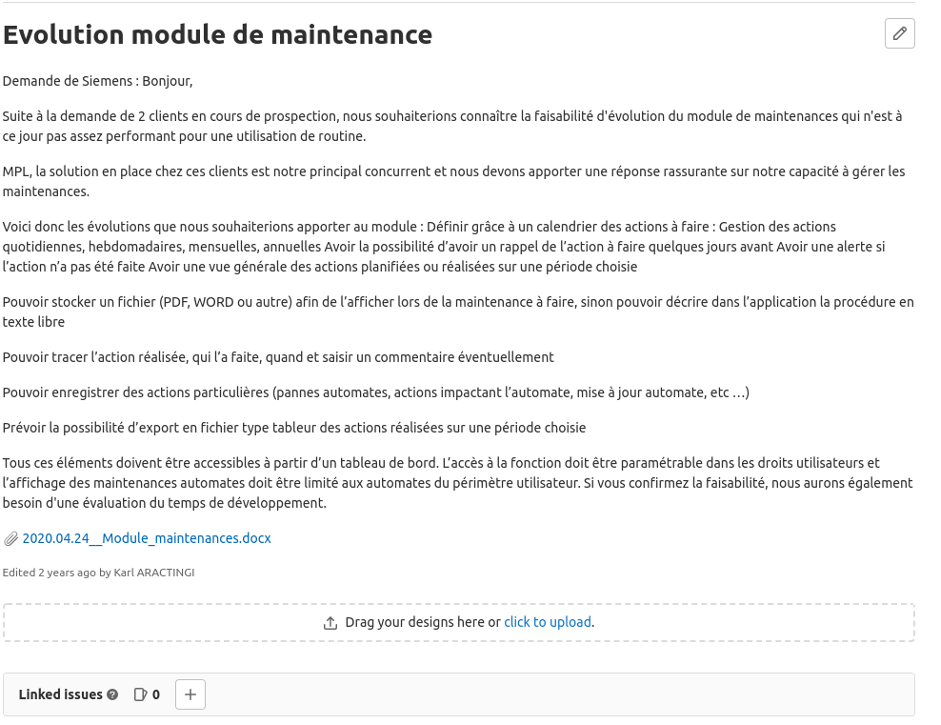
\includegraphics{images/issue_gitlab.png}
    \caption{Exemple d'une issue GitLab}
\end{figure}
\begin{figure}[hp]
    \centering
    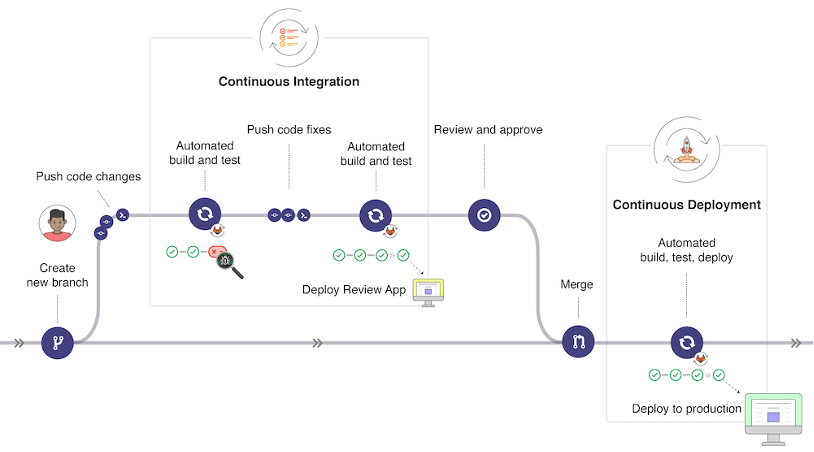
\includegraphics{images/cycle_gitlab.png}
    \caption{Le cycle de vie d'une issue Gitlab}
\end{figure}
\pagebreak

Afin de faciliter une bonne coordination au sein de l’équipe, GitLab propose un outil permettant de regrouper l’ensemble des issues ouvertes. Il s’agit du board.
C’est autour de lui que s’articule le Daily Meeting, ayant lieu chaque matin, au cours duquel sont passées en revues les issues.

En plus de donner une vue d’ensemble des issues ouvertes, il permet de voir rapidement à quels membres de l’équipe elles sont affectées, le temps estimé pour chaque issue et le temps réel qui y est passé ainsi que tous les deadlines à prendre en compte. 

Utilisé par l’équipe de développement mais également par l’équipe support ainsi que la chefferie de projet et de produit, cet outil simplifie grandement la communication entre les collaborateurs.
\begin{figure}[hp]
    \centering
    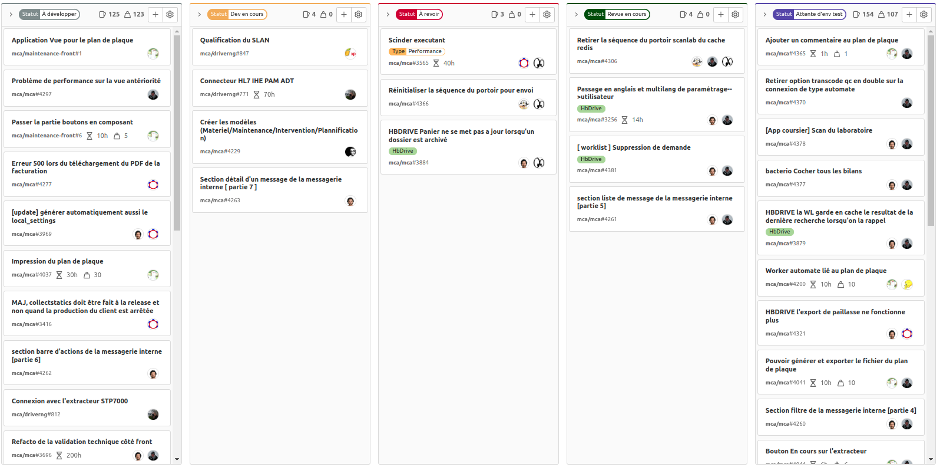
\includegraphics{images/board_gitlab.png}
    \caption{Exemple de Board GitLab}
\end{figure}

Le board proposé par GitLab pourrait être comparé à ceux utilisés dans la méthode agile Kanban. En effet, il s’agit pour Kanban d’un tableau consultable par l’ensemble des membres de l’équipe regroupant les tâches à faire, celles en cours ainsi que les tâches terminées.